\chapter{Background}
When designing the new Autograder front-end, it was necessary to develop other parts of the system for emulating dummy-data for the project. One of the most conventional ways of doing this is to create a database that stores the dummy-data, and have a server serve the front-end with that data. The system works in many ways as the fully functional Autograder, with predefined protocols for communications so that the new front-end can be implemented and deployed with a relatively small amount of effort. Making these protocols require us to both think about the current needs and future needs. Even though the system is currently up and running, many new ways of communicating with the new front-end is planned and will be implemented in the new system. It is however, no small task to create these sub-systems. We will go though some of the technologies we are using in this chapter.

\section{Front-end}s
One of the goals of the new Autograder front-end is to create a better and faster experience for the end-user. This means reflecting on the old design and expierence, and revisit the technologies and code written in the old Autograder front-end. This section describes the libraries and frameworks used for the new front-end.

\subsection{HTML, CSS and Bootstrap}
Hyper text markup language, or HTML, is a markup language used to build websites. Content is placed inside of different document object models, or DOM-elements. The different boxes of content is styled using a cascading style sheet, or CSS. Making the websites and layouts can take a lot of time. To simplify this, there are many open source project that supply off-the-shelf elements. Since we have experience with Bootstrap from earlier projects, it was decided that we would use Bootstrap 3.0 for the new front-end. The framework is in it's third iteration (soon 4th with Bootstrap 4.0 Alpha being shipped early 2016). The framework comes with build in styling, so the job of the designer (or rather lack of designers) is made easier. Compared to vanilla coding in HTML and CSS, the framework can remove countless of hours of coding, and the results look clean and functional. A grid system is also used for layout. The website is made responsive through a column-system that can change based on the client's screensize. The site becomes more mobile-friendy out of the box, however, it is not a fully optimized. The code must be tweaked to make the site optimized for all devices. With Autograder, the grid layout is used on all pages, but this will be covered in chapter \worry{Ref til chapter}

\todo{Lett inn referanser og alt sånt}

\subsection{ReactJS}
JavaScript is used to manipulate content on a website. Binding a data model and the DOM is necessary to have an always up-to-date website. Handlers for buttons and inputs are also handled in JavaScript. Handling all event listeners and functions connected to the DOM can be hard, especially when the application is as big as Autograder. Since the front-end communicates with a server, data will come in asynchronously and must trigger a re-render of the DOM-elements. This process of updating and binding data can be implemented using libraries such as ReactJS. React is an open source JavaScript library designed and maintained by Facebook \worry{ref here}. The library provides a view for data rendered as HTML, and maintains a state that can change depending on the data that comes from the server. This removes a lot of overhead programming for the developers. If the data in the server changes, the change are reflected on the page in real-time. Say for example that the users rights are changed from Student to Teacher. The front-end will have to reflect that change, and show data relevant for a teacher. With React, this change can be made without having to update the page manually. 

The choice between ReactJS and AngularJS (the other major JavaScript-library in the industry) is really based on preference. The component based pipeline that React offers is very appealing when the website will recycle a lot of the same elements. The new front-end can be compared to a single-page-application, where the different pages are loaded in without refreshing the page. Navigating between pages will therefore be very fast since the page will not be reloaded and the content up to date. Consequently, a lot of elements must be loaded and unloaded. React uses Virtual DOM to run its Tree Diff algorithm and figures out what parts of the DOM should be rendered, this enables quick re-rendering of only relevant for the change components. Components also hold methods such as \emph{componentWillMount()} and \emph{componentShouldMount()} to enable a greater control of data and elements being rendered on the page.

\begin{figure}[h]
\centering
\scalebox{0.5}{\scalefont{1.8}{% Graphic for TeX using PGF
% Title: /home/tomgli/workspace/github.com/bachopp/thesis/files/chapters/background/graphs/reactdiffdiagramthin.dia
% Creator: Dia v0.97.3
% CreationDate: Sat Apr 23 13:55:59 2016
% For: tomgli
% \usepackage{tikz}
% The following commands are not supported in PSTricks at present
% We define them conditionally, so when they are implemented,
% this pgf file will use them.
\ifx\du\undefined
  \newlength{\du}
\fi
\setlength{\du}{15\unitlength}
\begin{tikzpicture}
\pgftransformxscale{1.000000}
\pgftransformyscale{-1.000000}
\definecolor{dialinecolor}{rgb}{0.000000, 0.000000, 0.000000}
\pgfsetstrokecolor{dialinecolor}
\definecolor{dialinecolor}{rgb}{1.000000, 1.000000, 1.000000}
\pgfsetfillcolor{dialinecolor}
\definecolor{dialinecolor}{rgb}{1.000000, 1.000000, 1.000000}
\pgfsetfillcolor{dialinecolor}
\pgfpathellipse{\pgfpoint{34.909398\du}{57.597439\du}}{\pgfpoint{0.922067\du}{0\du}}{\pgfpoint{0\du}{0.874328\du}}
\pgfusepath{fill}
\pgfsetlinewidth{0.100000\du}
\pgfsetdash{}{0pt}
\pgfsetdash{}{0pt}
\pgfsetmiterjoin
\definecolor{dialinecolor}{rgb}{0.000000, 0.000000, 0.000000}
\pgfsetstrokecolor{dialinecolor}
\pgfpathellipse{\pgfpoint{34.909398\du}{57.597439\du}}{\pgfpoint{0.922067\du}{0\du}}{\pgfpoint{0\du}{0.874328\du}}
\pgfusepath{stroke}
% setfont left to latex
\definecolor{dialinecolor}{rgb}{0.000000, 0.000000, 0.000000}
\pgfsetstrokecolor{dialinecolor}
\node at (34.909398\du,57.792439\du){};
\definecolor{dialinecolor}{rgb}{1.000000, 1.000000, 1.000000}
\pgfsetfillcolor{dialinecolor}
\pgfpathellipse{\pgfpoint{34.925608\du}{60.858968\du}}{\pgfpoint{0.922067\du}{0\du}}{\pgfpoint{0\du}{0.874328\du}}
\pgfusepath{fill}
\pgfsetlinewidth{0.100000\du}
\pgfsetdash{}{0pt}
\pgfsetdash{}{0pt}
\pgfsetmiterjoin
\definecolor{dialinecolor}{rgb}{0.000000, 0.000000, 0.000000}
\pgfsetstrokecolor{dialinecolor}
\pgfpathellipse{\pgfpoint{34.925608\du}{60.858968\du}}{\pgfpoint{0.922067\du}{0\du}}{\pgfpoint{0\du}{0.874328\du}}
\pgfusepath{stroke}
% setfont left to latex
\definecolor{dialinecolor}{rgb}{0.000000, 0.000000, 0.000000}
\pgfsetstrokecolor{dialinecolor}
\node at (34.925608\du,61.053968\du){};
\definecolor{dialinecolor}{rgb}{1.000000, 1.000000, 1.000000}
\pgfsetfillcolor{dialinecolor}
\pgfpathellipse{\pgfpoint{39.675251\du}{57.895710\du}}{\pgfpoint{0.922067\du}{0\du}}{\pgfpoint{0\du}{0.874328\du}}
\pgfusepath{fill}
\pgfsetlinewidth{0.100000\du}
\pgfsetdash{}{0pt}
\pgfsetdash{}{0pt}
\pgfsetmiterjoin
\definecolor{dialinecolor}{rgb}{0.000000, 0.000000, 0.000000}
\pgfsetstrokecolor{dialinecolor}
\pgfpathellipse{\pgfpoint{39.675251\du}{57.895710\du}}{\pgfpoint{0.922067\du}{0\du}}{\pgfpoint{0\du}{0.874328\du}}
\pgfusepath{stroke}
% setfont left to latex
\definecolor{dialinecolor}{rgb}{0.000000, 0.000000, 0.000000}
\pgfsetstrokecolor{dialinecolor}
\node at (39.675251\du,58.090710\du){};
\definecolor{dialinecolor}{rgb}{1.000000, 0.509804, 0.509804}
\pgfsetfillcolor{dialinecolor}
\pgfpathellipse{\pgfpoint{38.686418\du}{62.486491\du}}{\pgfpoint{0.922067\du}{0\du}}{\pgfpoint{0\du}{0.874328\du}}
\pgfusepath{fill}
\pgfsetlinewidth{0.100000\du}
\pgfsetdash{}{0pt}
\pgfsetdash{}{0pt}
\pgfsetmiterjoin
\definecolor{dialinecolor}{rgb}{0.000000, 0.000000, 0.000000}
\pgfsetstrokecolor{dialinecolor}
\pgfpathellipse{\pgfpoint{38.686418\du}{62.486491\du}}{\pgfpoint{0.922067\du}{0\du}}{\pgfpoint{0\du}{0.874328\du}}
\pgfusepath{stroke}
% setfont left to latex
\definecolor{dialinecolor}{rgb}{0.000000, 0.000000, 0.000000}
\pgfsetstrokecolor{dialinecolor}
\node at (38.686418\du,62.681491\du){};
\definecolor{dialinecolor}{rgb}{0.898039, 0.898039, 0.898039}
\pgfsetfillcolor{dialinecolor}
\fill (48.025035\du,46.743799\du)--(48.025035\du,48.643799\du)--(51.299533\du,48.643799\du)--(51.299533\du,46.743799\du)--cycle;
\pgfsetlinewidth{0.100000\du}
\pgfsetdash{}{0pt}
\pgfsetdash{}{0pt}
\pgfsetmiterjoin
\definecolor{dialinecolor}{rgb}{0.549020, 0.549020, 0.549020}
\pgfsetstrokecolor{dialinecolor}
\draw (48.025035\du,46.743799\du)--(48.025035\du,48.643799\du)--(51.299533\du,48.643799\du)--(51.299533\du,46.743799\du)--cycle;
% setfont left to latex
\definecolor{dialinecolor}{rgb}{0.000000, 0.000000, 0.000000}
\pgfsetstrokecolor{dialinecolor}
\node at (49.662284\du,47.888799\du){};
\definecolor{dialinecolor}{rgb}{0.898039, 0.898039, 0.898039}
\pgfsetfillcolor{dialinecolor}
\fill (46.210841\du,49.629967\du)--(46.210841\du,51.529967\du)--(49.485338\du,51.529967\du)--(49.485338\du,49.629967\du)--cycle;
\pgfsetlinewidth{0.100000\du}
\pgfsetdash{}{0pt}
\pgfsetdash{}{0pt}
\pgfsetmiterjoin
\definecolor{dialinecolor}{rgb}{0.549020, 0.549020, 0.549020}
\pgfsetstrokecolor{dialinecolor}
\draw (46.210841\du,49.629967\du)--(46.210841\du,51.529967\du)--(49.485338\du,51.529967\du)--(49.485338\du,49.629967\du)--cycle;
% setfont left to latex
\definecolor{dialinecolor}{rgb}{0.000000, 0.000000, 0.000000}
\pgfsetstrokecolor{dialinecolor}
\node at (47.848090\du,50.774967\du){};
\definecolor{dialinecolor}{rgb}{0.898039, 0.898039, 0.898039}
\pgfsetfillcolor{dialinecolor}
\fill (50.571434\du,49.649420\du)--(50.571434\du,51.549420\du)--(53.845932\du,51.549420\du)--(53.845932\du,49.649420\du)--cycle;
\pgfsetlinewidth{0.100000\du}
\pgfsetdash{}{0pt}
\pgfsetdash{}{0pt}
\pgfsetmiterjoin
\definecolor{dialinecolor}{rgb}{0.549020, 0.549020, 0.549020}
\pgfsetstrokecolor{dialinecolor}
\draw (50.571434\du,49.649420\du)--(50.571434\du,51.549420\du)--(53.845932\du,51.549420\du)--(53.845932\du,49.649420\du)--cycle;
% setfont left to latex
\definecolor{dialinecolor}{rgb}{0.000000, 0.000000, 0.000000}
\pgfsetstrokecolor{dialinecolor}
\node at (52.208683\du,50.794420\du){};
\definecolor{dialinecolor}{rgb}{0.898039, 0.898039, 0.898039}
\pgfsetfillcolor{dialinecolor}
\fill (44.038649\du,52.385733\du)--(44.038649\du,54.285733\du)--(47.313147\du,54.285733\du)--(47.313147\du,52.385733\du)--cycle;
\pgfsetlinewidth{0.100000\du}
\pgfsetdash{}{0pt}
\pgfsetdash{}{0pt}
\pgfsetmiterjoin
\definecolor{dialinecolor}{rgb}{0.549020, 0.549020, 0.549020}
\pgfsetstrokecolor{dialinecolor}
\draw (44.038649\du,52.385733\du)--(44.038649\du,54.285733\du)--(47.313147\du,54.285733\du)--(47.313147\du,52.385733\du)--cycle;
% setfont left to latex
\definecolor{dialinecolor}{rgb}{0.000000, 0.000000, 0.000000}
\pgfsetstrokecolor{dialinecolor}
\node at (45.675898\du,53.530733\du){};
\definecolor{dialinecolor}{rgb}{0.898039, 0.898039, 0.898039}
\pgfsetfillcolor{dialinecolor}
\fill (48.399243\du,52.405185\du)--(48.399243\du,54.305185\du)--(51.673740\du,54.305185\du)--(51.673740\du,52.405185\du)--cycle;
\pgfsetlinewidth{0.100000\du}
\pgfsetdash{}{0pt}
\pgfsetdash{}{0pt}
\pgfsetmiterjoin
\definecolor{dialinecolor}{rgb}{0.549020, 0.549020, 0.549020}
\pgfsetstrokecolor{dialinecolor}
\draw (48.399243\du,52.405185\du)--(48.399243\du,54.305185\du)--(51.673740\du,54.305185\du)--(51.673740\du,52.405185\du)--cycle;
% setfont left to latex
\definecolor{dialinecolor}{rgb}{0.000000, 0.000000, 0.000000}
\pgfsetstrokecolor{dialinecolor}
\node at (50.036492\du,53.550185\du){};
\definecolor{dialinecolor}{rgb}{0.898039, 0.898039, 0.898039}
\pgfsetfillcolor{dialinecolor}
\fill (48.512715\du,55.368444\du)--(48.512715\du,57.268444\du)--(51.787213\du,57.268444\du)--(51.787213\du,55.368444\du)--cycle;
\pgfsetlinewidth{0.100000\du}
\pgfsetdash{}{0pt}
\pgfsetdash{}{0pt}
\pgfsetmiterjoin
\definecolor{dialinecolor}{rgb}{0.549020, 0.549020, 0.549020}
\pgfsetstrokecolor{dialinecolor}
\draw (48.512715\du,55.368444\du)--(48.512715\du,57.268444\du)--(51.787213\du,57.268444\du)--(51.787213\du,55.368444\du)--cycle;
% setfont left to latex
\definecolor{dialinecolor}{rgb}{0.000000, 0.000000, 0.000000}
\pgfsetstrokecolor{dialinecolor}
\node at (50.149964\du,56.513444\du){};
\definecolor{dialinecolor}{rgb}{1.000000, 1.000000, 1.000000}
\pgfsetfillcolor{dialinecolor}
\pgfpathellipse{\pgfpoint{31.922753\du}{56.062026\du}}{\pgfpoint{0.922067\du}{0\du}}{\pgfpoint{0\du}{0.874328\du}}
\pgfusepath{fill}
\pgfsetlinewidth{0.100000\du}
\pgfsetdash{}{0pt}
\pgfsetdash{}{0pt}
\pgfsetmiterjoin
\definecolor{dialinecolor}{rgb}{0.000000, 0.000000, 0.000000}
\pgfsetstrokecolor{dialinecolor}
\pgfpathellipse{\pgfpoint{31.922753\du}{56.062026\du}}{\pgfpoint{0.922067\du}{0\du}}{\pgfpoint{0\du}{0.874328\du}}
\pgfusepath{stroke}
% setfont left to latex
\definecolor{dialinecolor}{rgb}{0.000000, 0.000000, 0.000000}
\pgfsetstrokecolor{dialinecolor}
\node at (31.922753\du,56.257026\du){};
\definecolor{dialinecolor}{rgb}{0.898039, 0.898039, 0.898039}
\pgfsetfillcolor{dialinecolor}
\fill (47.984149\du,61.262534\du)--(47.984149\du,63.162534\du)--(51.258647\du,63.162534\du)--(51.258647\du,61.262534\du)--cycle;
\pgfsetlinewidth{0.100000\du}
\pgfsetdash{}{0pt}
\pgfsetdash{}{0pt}
\pgfsetmiterjoin
\definecolor{dialinecolor}{rgb}{0.549020, 0.549020, 0.549020}
\pgfsetstrokecolor{dialinecolor}
\draw (47.984149\du,61.262534\du)--(47.984149\du,63.162534\du)--(51.258647\du,63.162534\du)--(51.258647\du,61.262534\du)--cycle;
% setfont left to latex
\definecolor{dialinecolor}{rgb}{0.000000, 0.000000, 0.000000}
\pgfsetstrokecolor{dialinecolor}
\node at (49.621398\du,62.407534\du){};
\definecolor{dialinecolor}{rgb}{0.898039, 0.898039, 0.898039}
\pgfsetfillcolor{dialinecolor}
\fill (46.169955\du,64.148703\du)--(46.169955\du,66.048703\du)--(49.444453\du,66.048703\du)--(49.444453\du,64.148703\du)--cycle;
\pgfsetlinewidth{0.100000\du}
\pgfsetdash{}{0pt}
\pgfsetdash{}{0pt}
\pgfsetmiterjoin
\definecolor{dialinecolor}{rgb}{0.549020, 0.549020, 0.549020}
\pgfsetstrokecolor{dialinecolor}
\draw (46.169955\du,64.148703\du)--(46.169955\du,66.048703\du)--(49.444453\du,66.048703\du)--(49.444453\du,64.148703\du)--cycle;
% setfont left to latex
\definecolor{dialinecolor}{rgb}{0.000000, 0.000000, 0.000000}
\pgfsetstrokecolor{dialinecolor}
\node at (47.807204\du,65.293703\du){};
\definecolor{dialinecolor}{rgb}{0.898039, 0.898039, 0.898039}
\pgfsetfillcolor{dialinecolor}
\fill (50.530549\du,64.168155\du)--(50.530549\du,66.068155\du)--(53.805046\du,66.068155\du)--(53.805046\du,64.168155\du)--cycle;
\pgfsetlinewidth{0.100000\du}
\pgfsetdash{}{0pt}
\pgfsetdash{}{0pt}
\pgfsetmiterjoin
\definecolor{dialinecolor}{rgb}{0.549020, 0.549020, 0.549020}
\pgfsetstrokecolor{dialinecolor}
\draw (50.530549\du,64.168155\du)--(50.530549\du,66.068155\du)--(53.805046\du,66.068155\du)--(53.805046\du,64.168155\du)--cycle;
% setfont left to latex
\definecolor{dialinecolor}{rgb}{0.000000, 0.000000, 0.000000}
\pgfsetstrokecolor{dialinecolor}
\node at (52.167798\du,65.313155\du){};
\definecolor{dialinecolor}{rgb}{1.000000, 0.509804, 0.509804}
\pgfsetfillcolor{dialinecolor}
\fill (43.997764\du,66.904468\du)--(43.997764\du,68.804468\du)--(47.272261\du,68.804468\du)--(47.272261\du,66.904468\du)--cycle;
\pgfsetlinewidth{0.100000\du}
\pgfsetdash{}{0pt}
\pgfsetdash{}{0pt}
\pgfsetmiterjoin
\definecolor{dialinecolor}{rgb}{0.549020, 0.549020, 0.549020}
\pgfsetstrokecolor{dialinecolor}
\draw (43.997764\du,66.904468\du)--(43.997764\du,68.804468\du)--(47.272261\du,68.804468\du)--(47.272261\du,66.904468\du)--cycle;
% setfont left to latex
\definecolor{dialinecolor}{rgb}{0.000000, 0.000000, 0.000000}
\pgfsetstrokecolor{dialinecolor}
\node at (45.635013\du,68.049468\du){};
\definecolor{dialinecolor}{rgb}{0.898039, 0.898039, 0.898039}
\pgfsetfillcolor{dialinecolor}
\fill (48.358357\du,66.923920\du)--(48.358357\du,68.823920\du)--(51.632855\du,68.823920\du)--(51.632855\du,66.923920\du)--cycle;
\pgfsetlinewidth{0.100000\du}
\pgfsetdash{}{0pt}
\pgfsetdash{}{0pt}
\pgfsetmiterjoin
\definecolor{dialinecolor}{rgb}{0.549020, 0.549020, 0.549020}
\pgfsetstrokecolor{dialinecolor}
\draw (48.358357\du,66.923920\du)--(48.358357\du,68.823920\du)--(51.632855\du,68.823920\du)--(51.632855\du,66.923920\du)--cycle;
% setfont left to latex
\definecolor{dialinecolor}{rgb}{0.000000, 0.000000, 0.000000}
\pgfsetstrokecolor{dialinecolor}
\node at (49.995606\du,68.068920\du){};
\definecolor{dialinecolor}{rgb}{0.898039, 0.898039, 0.898039}
\pgfsetfillcolor{dialinecolor}
\fill (48.471830\du,69.887179\du)--(48.471830\du,71.787179\du)--(51.746328\du,71.787179\du)--(51.746328\du,69.887179\du)--cycle;
\pgfsetlinewidth{0.100000\du}
\pgfsetdash{}{0pt}
\pgfsetdash{}{0pt}
\pgfsetmiterjoin
\definecolor{dialinecolor}{rgb}{0.549020, 0.549020, 0.549020}
\pgfsetstrokecolor{dialinecolor}
\draw (48.471830\du,69.887179\du)--(48.471830\du,71.787179\du)--(51.746328\du,71.787179\du)--(51.746328\du,69.887179\du)--cycle;
% setfont left to latex
\definecolor{dialinecolor}{rgb}{0.000000, 0.000000, 0.000000}
\pgfsetstrokecolor{dialinecolor}
\node at (50.109079\du,71.032179\du){};
\definecolor{dialinecolor}{rgb}{1.000000, 1.000000, 1.000000}
\pgfsetfillcolor{dialinecolor}
\fill (67.651782\du,54.752294\du)--(67.651782\du,56.652294\du)--(70.926279\du,56.652294\du)--(70.926279\du,54.752294\du)--cycle;
\pgfsetlinewidth{0.100000\du}
\pgfsetdash{}{0pt}
\pgfsetdash{}{0pt}
\pgfsetmiterjoin
\definecolor{dialinecolor}{rgb}{0.000000, 0.000000, 0.000000}
\pgfsetstrokecolor{dialinecolor}
\draw (67.651782\du,54.752294\du)--(67.651782\du,56.652294\du)--(70.926279\du,56.652294\du)--(70.926279\du,54.752294\du)--cycle;
% setfont left to latex
\definecolor{dialinecolor}{rgb}{0.000000, 0.000000, 0.000000}
\pgfsetstrokecolor{dialinecolor}
\node at (69.289030\du,55.897294\du){};
\definecolor{dialinecolor}{rgb}{1.000000, 1.000000, 1.000000}
\pgfsetfillcolor{dialinecolor}
\fill (65.837587\du,57.638463\du)--(65.837587\du,59.538463\du)--(69.112085\du,59.538463\du)--(69.112085\du,57.638463\du)--cycle;
\pgfsetlinewidth{0.100000\du}
\pgfsetdash{}{0pt}
\pgfsetdash{}{0pt}
\pgfsetmiterjoin
\definecolor{dialinecolor}{rgb}{0.000000, 0.000000, 0.000000}
\pgfsetstrokecolor{dialinecolor}
\draw (65.837587\du,57.638463\du)--(65.837587\du,59.538463\du)--(69.112085\du,59.538463\du)--(69.112085\du,57.638463\du)--cycle;
% setfont left to latex
\definecolor{dialinecolor}{rgb}{0.000000, 0.000000, 0.000000}
\pgfsetstrokecolor{dialinecolor}
\node at (67.474836\du,58.783463\du){};
\definecolor{dialinecolor}{rgb}{1.000000, 1.000000, 1.000000}
\pgfsetfillcolor{dialinecolor}
\fill (70.198181\du,57.657915\du)--(70.198181\du,59.557915\du)--(73.472679\du,59.557915\du)--(73.472679\du,57.657915\du)--cycle;
\pgfsetlinewidth{0.100000\du}
\pgfsetdash{}{0pt}
\pgfsetdash{}{0pt}
\pgfsetmiterjoin
\definecolor{dialinecolor}{rgb}{0.000000, 0.000000, 0.000000}
\pgfsetstrokecolor{dialinecolor}
\draw (70.198181\du,57.657915\du)--(70.198181\du,59.557915\du)--(73.472679\du,59.557915\du)--(73.472679\du,57.657915\du)--cycle;
% setfont left to latex
\definecolor{dialinecolor}{rgb}{0.000000, 0.000000, 0.000000}
\pgfsetstrokecolor{dialinecolor}
\node at (71.835430\du,58.802915\du){};
\definecolor{dialinecolor}{rgb}{1.000000, 0.509804, 0.509804}
\pgfsetfillcolor{dialinecolor}
\fill (63.665396\du,60.394228\du)--(63.665396\du,62.294228\du)--(66.939894\du,62.294228\du)--(66.939894\du,60.394228\du)--cycle;
\pgfsetlinewidth{0.100000\du}
\pgfsetdash{}{0pt}
\pgfsetdash{}{0pt}
\pgfsetmiterjoin
\definecolor{dialinecolor}{rgb}{0.000000, 0.000000, 0.000000}
\pgfsetstrokecolor{dialinecolor}
\draw (63.665396\du,60.394228\du)--(63.665396\du,62.294228\du)--(66.939894\du,62.294228\du)--(66.939894\du,60.394228\du)--cycle;
% setfont left to latex
\definecolor{dialinecolor}{rgb}{0.000000, 0.000000, 0.000000}
\pgfsetstrokecolor{dialinecolor}
\node at (65.302645\du,61.539228\du){};
\definecolor{dialinecolor}{rgb}{1.000000, 1.000000, 1.000000}
\pgfsetfillcolor{dialinecolor}
\fill (68.025989\du,60.413680\du)--(68.025989\du,62.313680\du)--(71.300487\du,62.313680\du)--(71.300487\du,60.413680\du)--cycle;
\pgfsetlinewidth{0.100000\du}
\pgfsetdash{}{0pt}
\pgfsetdash{}{0pt}
\pgfsetmiterjoin
\definecolor{dialinecolor}{rgb}{0.000000, 0.000000, 0.000000}
\pgfsetstrokecolor{dialinecolor}
\draw (68.025989\du,60.413680\du)--(68.025989\du,62.313680\du)--(71.300487\du,62.313680\du)--(71.300487\du,60.413680\du)--cycle;
% setfont left to latex
\definecolor{dialinecolor}{rgb}{0.000000, 0.000000, 0.000000}
\pgfsetstrokecolor{dialinecolor}
\node at (69.663238\du,61.558680\du){};
\definecolor{dialinecolor}{rgb}{1.000000, 1.000000, 1.000000}
\pgfsetfillcolor{dialinecolor}
\fill (68.139462\du,63.376939\du)--(68.139462\du,65.276939\du)--(71.413960\du,65.276939\du)--(71.413960\du,63.376939\du)--cycle;
\pgfsetlinewidth{0.100000\du}
\pgfsetdash{}{0pt}
\pgfsetdash{}{0pt}
\pgfsetmiterjoin
\definecolor{dialinecolor}{rgb}{0.000000, 0.000000, 0.000000}
\pgfsetstrokecolor{dialinecolor}
\draw (68.139462\du,63.376939\du)--(68.139462\du,65.276939\du)--(71.413960\du,65.276939\du)--(71.413960\du,63.376939\du)--cycle;
% setfont left to latex
\definecolor{dialinecolor}{rgb}{0.000000, 0.000000, 0.000000}
\pgfsetstrokecolor{dialinecolor}
\node at (69.776711\du,64.521939\du){};
\pgfsetlinewidth{0.100000\du}
\pgfsetdash{}{0pt}
\pgfsetdash{}{0pt}
\pgfsetmiterjoin
\definecolor{dialinecolor}{rgb}{0.549020, 0.549020, 0.549020}
\pgfsetstrokecolor{dialinecolor}
\pgfpathellipse{\pgfpoint{49.127059\du}{51.603158\du}}{\pgfpoint{6.946203\du}{0\du}}{\pgfpoint{0\du}{6.480362\du}}
\pgfusepath{stroke}
% setfont left to latex
\definecolor{dialinecolor}{rgb}{0.000000, 0.000000, 0.000000}
\pgfsetstrokecolor{dialinecolor}
\node at (49.127059\du,51.798158\du){};
\pgfsetlinewidth{0.100000\du}
\pgfsetdash{}{0pt}
\pgfsetdash{}{0pt}
\pgfsetbuttcap
{
\definecolor{dialinecolor}{rgb}{0.549020, 0.549020, 0.549020}
\pgfsetfillcolor{dialinecolor}
% was here!!!
\definecolor{dialinecolor}{rgb}{0.549020, 0.549020, 0.549020}
\pgfsetstrokecolor{dialinecolor}
\draw (49.034225\du,48.692966\du)--(48.476148\du,49.580801\du);
}
\pgfsetlinewidth{0.100000\du}
\pgfsetdash{}{0pt}
\pgfsetdash{}{0pt}
\pgfsetbuttcap
{
\definecolor{dialinecolor}{rgb}{0.549020, 0.549020, 0.549020}
\pgfsetfillcolor{dialinecolor}
% was here!!!
\definecolor{dialinecolor}{rgb}{0.549020, 0.549020, 0.549020}
\pgfsetstrokecolor{dialinecolor}
\draw (50.538230\du,48.693315\du)--(51.332737\du,49.599903\du);
}
\pgfsetlinewidth{0.100000\du}
\pgfsetdash{}{0pt}
\pgfsetdash{}{0pt}
\pgfsetbuttcap
{
\definecolor{dialinecolor}{rgb}{0.549020, 0.549020, 0.549020}
\pgfsetfillcolor{dialinecolor}
% was here!!!
\definecolor{dialinecolor}{rgb}{0.549020, 0.549020, 0.549020}
\pgfsetstrokecolor{dialinecolor}
\draw (47.059769\du,51.580076\du)--(46.464219\du,52.335624\du);
}
\pgfsetlinewidth{0.100000\du}
\pgfsetdash{}{0pt}
\pgfsetdash{}{0pt}
\pgfsetbuttcap
{
\definecolor{dialinecolor}{rgb}{0.549020, 0.549020, 0.549020}
\pgfsetfillcolor{dialinecolor}
% was here!!!
\definecolor{dialinecolor}{rgb}{0.549020, 0.549020, 0.549020}
\pgfsetstrokecolor{dialinecolor}
\draw (48.635615\du,51.578666\du)--(49.248966\du,52.356486\du);
}
\pgfsetlinewidth{0.100000\du}
\pgfsetdash{}{0pt}
\pgfsetdash{}{0pt}
\pgfsetbuttcap
{
\definecolor{dialinecolor}{rgb}{0.549020, 0.549020, 0.549020}
\pgfsetfillcolor{dialinecolor}
% was here!!!
\definecolor{dialinecolor}{rgb}{0.549020, 0.549020, 0.549020}
\pgfsetstrokecolor{dialinecolor}
\draw (50.074791\du,54.355357\du)--(50.111664\du,55.318272\du);
}
\pgfsetlinewidth{0.100000\du}
\pgfsetdash{}{0pt}
\pgfsetdash{}{0pt}
\pgfsetbuttcap
{
\definecolor{dialinecolor}{rgb}{0.549020, 0.549020, 0.549020}
\pgfsetfillcolor{dialinecolor}
% was here!!!
\definecolor{dialinecolor}{rgb}{0.549020, 0.549020, 0.549020}
\pgfsetstrokecolor{dialinecolor}
\draw (48.993340\du,63.211701\du)--(48.435263\du,64.099536\du);
}
\pgfsetlinewidth{0.100000\du}
\pgfsetdash{}{0pt}
\pgfsetdash{}{0pt}
\pgfsetbuttcap
{
\definecolor{dialinecolor}{rgb}{0.549020, 0.549020, 0.549020}
\pgfsetfillcolor{dialinecolor}
% was here!!!
\definecolor{dialinecolor}{rgb}{0.549020, 0.549020, 0.549020}
\pgfsetstrokecolor{dialinecolor}
\draw (50.497345\du,63.212051\du)--(51.291851\du,64.118638\du);
}
\pgfsetlinewidth{0.100000\du}
\pgfsetdash{}{0pt}
\pgfsetdash{}{0pt}
\pgfsetbuttcap
{
\definecolor{dialinecolor}{rgb}{0.549020, 0.549020, 0.549020}
\pgfsetfillcolor{dialinecolor}
% was here!!!
\definecolor{dialinecolor}{rgb}{0.549020, 0.549020, 0.549020}
\pgfsetstrokecolor{dialinecolor}
\draw (47.018883\du,66.098811\du)--(46.423334\du,66.854359\du);
}
\pgfsetlinewidth{0.100000\du}
\pgfsetdash{}{0pt}
\pgfsetdash{}{0pt}
\pgfsetbuttcap
{
\definecolor{dialinecolor}{rgb}{0.549020, 0.549020, 0.549020}
\pgfsetfillcolor{dialinecolor}
% was here!!!
\definecolor{dialinecolor}{rgb}{0.549020, 0.549020, 0.549020}
\pgfsetstrokecolor{dialinecolor}
\draw (48.594730\du,66.097402\du)--(49.208081\du,66.875221\du);
}
\pgfsetlinewidth{0.100000\du}
\pgfsetdash{}{0pt}
\pgfsetdash{}{0pt}
\pgfsetbuttcap
{
\definecolor{dialinecolor}{rgb}{0.549020, 0.549020, 0.549020}
\pgfsetfillcolor{dialinecolor}
% was here!!!
\definecolor{dialinecolor}{rgb}{0.549020, 0.549020, 0.549020}
\pgfsetstrokecolor{dialinecolor}
\draw (50.033906\du,68.874092\du)--(50.070779\du,69.837007\du);
}
\pgfsetlinewidth{0.100000\du}
\pgfsetdash{}{0pt}
\pgfsetdash{}{0pt}
\pgfsetbuttcap
{
\definecolor{dialinecolor}{rgb}{0.000000, 0.000000, 0.000000}
\pgfsetfillcolor{dialinecolor}
% was here!!!
\definecolor{dialinecolor}{rgb}{0.000000, 0.000000, 0.000000}
\pgfsetstrokecolor{dialinecolor}
\draw (68.660972\du,56.701461\du)--(68.102895\du,57.589296\du);
}
\pgfsetlinewidth{0.100000\du}
\pgfsetdash{}{0pt}
\pgfsetdash{}{0pt}
\pgfsetbuttcap
{
\definecolor{dialinecolor}{rgb}{0.000000, 0.000000, 0.000000}
\pgfsetfillcolor{dialinecolor}
% was here!!!
\definecolor{dialinecolor}{rgb}{0.000000, 0.000000, 0.000000}
\pgfsetstrokecolor{dialinecolor}
\draw (70.164977\du,56.701811\du)--(70.959483\du,57.608398\du);
}
\pgfsetlinewidth{0.100000\du}
\pgfsetdash{}{0pt}
\pgfsetdash{}{0pt}
\pgfsetbuttcap
{
\definecolor{dialinecolor}{rgb}{0.000000, 0.000000, 0.000000}
\pgfsetfillcolor{dialinecolor}
% was here!!!
\definecolor{dialinecolor}{rgb}{0.000000, 0.000000, 0.000000}
\pgfsetstrokecolor{dialinecolor}
\draw (66.686515\du,59.588571\du)--(66.090966\du,60.344119\du);
}
\pgfsetlinewidth{0.100000\du}
\pgfsetdash{}{0pt}
\pgfsetdash{}{0pt}
\pgfsetbuttcap
{
\definecolor{dialinecolor}{rgb}{0.000000, 0.000000, 0.000000}
\pgfsetfillcolor{dialinecolor}
% was here!!!
\definecolor{dialinecolor}{rgb}{0.000000, 0.000000, 0.000000}
\pgfsetstrokecolor{dialinecolor}
\draw (68.262362\du,59.587162\du)--(68.875713\du,60.364981\du);
}
\pgfsetlinewidth{0.100000\du}
\pgfsetdash{}{0pt}
\pgfsetdash{}{0pt}
\pgfsetbuttcap
{
\definecolor{dialinecolor}{rgb}{0.000000, 0.000000, 0.000000}
\pgfsetfillcolor{dialinecolor}
% was here!!!
\definecolor{dialinecolor}{rgb}{0.000000, 0.000000, 0.000000}
\pgfsetstrokecolor{dialinecolor}
\draw (69.701538\du,62.363852\du)--(69.738411\du,63.326767\du);
}
\definecolor{dialinecolor}{rgb}{1.000000, 0.509804, 0.509804}
\pgfsetfillcolor{dialinecolor}
\fill (56.489531\du,58.272316\du)--(56.489531\du,60.172316\du)--(59.764029\du,60.172316\du)--(59.764029\du,58.272316\du)--cycle;
\pgfsetlinewidth{0.100000\du}
\pgfsetdash{}{0pt}
\pgfsetdash{}{0pt}
\pgfsetmiterjoin
\definecolor{dialinecolor}{rgb}{0.000000, 0.000000, 0.000000}
\pgfsetstrokecolor{dialinecolor}
\draw (56.489531\du,58.272316\du)--(56.489531\du,60.172316\du)--(59.764029\du,60.172316\du)--(59.764029\du,58.272316\du)--cycle;
% setfont left to latex
\definecolor{dialinecolor}{rgb}{0.000000, 0.000000, 0.000000}
\pgfsetstrokecolor{dialinecolor}
\node at (58.126780\du,59.417316\du){};
\pgfsetlinewidth{0.100000\du}
\pgfsetdash{}{0pt}
\pgfsetdash{}{0pt}
\pgfsetmiterjoin
\definecolor{dialinecolor}{rgb}{0.549020, 0.549020, 0.549020}
\pgfsetstrokecolor{dialinecolor}
\pgfpathellipse{\pgfpoint{49.286190\du}{66.757518\du}}{\pgfpoint{6.946203\du}{0\du}}{\pgfpoint{0\du}{6.480362\du}}
\pgfusepath{stroke}
% setfont left to latex
\definecolor{dialinecolor}{rgb}{0.000000, 0.000000, 0.000000}
\pgfsetstrokecolor{dialinecolor}
\node at (49.286190\du,66.952518\du){};
\pgfsetlinewidth{0.100000\du}
\pgfsetdash{}{0pt}
\pgfsetdash{}{0pt}
\pgfsetbuttcap
{
\definecolor{dialinecolor}{rgb}{0.000000, 0.000000, 0.000000}
\pgfsetfillcolor{dialinecolor}
% was here!!!
\definecolor{dialinecolor}{rgb}{0.000000, 0.000000, 0.000000}
\pgfsetstrokecolor{dialinecolor}
\draw (32.777695\du,56.501546\du)--(34.054456\du,57.157920\du);
}
\pgfsetlinewidth{0.100000\du}
\pgfsetdash{}{0pt}
\pgfsetdash{}{0pt}
\pgfsetbuttcap
{
\definecolor{dialinecolor}{rgb}{0.000000, 0.000000, 0.000000}
\pgfsetfillcolor{dialinecolor}
% was here!!!
\definecolor{dialinecolor}{rgb}{0.000000, 0.000000, 0.000000}
\pgfsetstrokecolor{dialinecolor}
\draw (35.878625\du,57.658098\du)--(38.706024\du,57.835051\du);
}
\pgfsetlinewidth{0.100000\du}
\pgfsetdash{}{0pt}
\pgfsetdash{}{0pt}
\pgfsetbuttcap
{
\definecolor{dialinecolor}{rgb}{0.000000, 0.000000, 0.000000}
\pgfsetfillcolor{dialinecolor}
% was here!!!
\definecolor{dialinecolor}{rgb}{0.000000, 0.000000, 0.000000}
\pgfsetstrokecolor{dialinecolor}
\draw (34.913993\du,58.521911\du)--(34.921014\du,59.934497\du);
}
\pgfsetlinewidth{0.100000\du}
\pgfsetdash{}{0pt}
\pgfsetdash{}{0pt}
\pgfsetbuttcap
{
\definecolor{dialinecolor}{rgb}{0.000000, 0.000000, 0.000000}
\pgfsetfillcolor{dialinecolor}
% was here!!!
\definecolor{dialinecolor}{rgb}{0.000000, 0.000000, 0.000000}
\pgfsetstrokecolor{dialinecolor}
\draw (39.481154\du,58.796830\du)--(38.880515\du,61.585371\du);
}
\pgfsetlinewidth{0.100000\du}
\pgfsetdash{}{0pt}
\pgfsetdash{}{0pt}
\pgfsetbuttcap
{
\definecolor{dialinecolor}{rgb}{0.000000, 0.000000, 0.000000}
\pgfsetfillcolor{dialinecolor}
% was here!!!
\definecolor{dialinecolor}{rgb}{0.000000, 0.000000, 0.000000}
\pgfsetstrokecolor{dialinecolor}
\draw (35.808884\du,61.241214\du)--(37.803142\du,62.104246\du);
}
\pgfsetlinewidth{0.100000\du}
\pgfsetdash{}{0pt}
\pgfsetdash{}{0pt}
\pgfsetbuttcap
{
\definecolor{dialinecolor}{rgb}{1.000000, 0.509804, 0.509804}
\pgfsetfillcolor{dialinecolor}
% was here!!!
\pgfsetarrowsend{latex}
\definecolor{dialinecolor}{rgb}{1.000000, 0.509804, 0.509804}
\pgfsetstrokecolor{dialinecolor}
\draw (54.147866\du,56.151163\du)--(56.489531\du,58.272316\du);
}
\pgfsetlinewidth{0.100000\du}
\pgfsetdash{}{0pt}
\pgfsetdash{}{0pt}
\pgfsetbuttcap
{
\definecolor{dialinecolor}{rgb}{1.000000, 0.509804, 0.509804}
\pgfsetfillcolor{dialinecolor}
% was here!!!
\pgfsetarrowsend{latex}
\definecolor{dialinecolor}{rgb}{1.000000, 0.509804, 0.509804}
\pgfsetstrokecolor{dialinecolor}
\draw (54.197898\du,62.175211\du)--(56.489531\du,60.172316\du);
}
\pgfsetlinewidth{0.100000\du}
\pgfsetdash{}{0pt}
\pgfsetdash{}{0pt}
\pgfsetbuttcap
{
\definecolor{dialinecolor}{rgb}{1.000000, 0.509804, 0.509804}
\pgfsetfillcolor{dialinecolor}
% was here!!!
\pgfsetarrowsend{latex}
\definecolor{dialinecolor}{rgb}{1.000000, 0.509804, 0.509804}
\pgfsetstrokecolor{dialinecolor}
\draw (59.764029\du,59.222316\du)--(63.665396\du,60.394228\du);
}
\pgfsetlinewidth{0.100000\du}
\pgfsetdash{}{0pt}
\pgfsetdash{}{0pt}
\pgfsetbuttcap
{
\definecolor{dialinecolor}{rgb}{0.898039, 0.898039, 0.898039}
\pgfsetfillcolor{dialinecolor}
% was here!!!
\definecolor{dialinecolor}{rgb}{0.898039, 0.898039, 0.898039}
\pgfsetstrokecolor{dialinecolor}
\draw (30.974207\du,51.876227\du)--(51.944387\du,60.770445\du);
}
\pgfsetlinewidth{0.100000\du}
\pgfsetdash{}{0pt}
\pgfsetdash{}{0pt}
\pgfsetbuttcap
{
\definecolor{dialinecolor}{rgb}{0.898039, 0.898039, 0.898039}
\pgfsetfillcolor{dialinecolor}
% was here!!!
\definecolor{dialinecolor}{rgb}{0.898039, 0.898039, 0.898039}
\pgfsetstrokecolor{dialinecolor}
\draw (31.629635\du,67.105300\du)--(51.785256\du,57.590232\du);
}
\pgfsetlinewidth{0.100000\du}
\pgfsetdash{}{0pt}
\pgfsetdash{}{0pt}
\pgfsetbuttcap
{
\definecolor{dialinecolor}{rgb}{0.898039, 0.898039, 0.898039}
\pgfsetfillcolor{dialinecolor}
% was here!!!
\definecolor{dialinecolor}{rgb}{0.898039, 0.898039, 0.898039}
\pgfsetstrokecolor{dialinecolor}
\draw (44.374483\du,71.339826\du)--(29.046476\du,59.355822\du);
}
\pgfsetlinewidth{0.100000\du}
\pgfsetdash{}{0pt}
\pgfsetdash{}{0pt}
\pgfsetbuttcap
{
\definecolor{dialinecolor}{rgb}{0.898039, 0.898039, 0.898039}
\pgfsetfillcolor{dialinecolor}
% was here!!!
\definecolor{dialinecolor}{rgb}{0.898039, 0.898039, 0.898039}
\pgfsetstrokecolor{dialinecolor}
\draw (44.215351\du,47.020850\du)--(28.930812\du,56.541335\du);
}
% setfont left to latex
\definecolor{dialinecolor}{rgb}{0.000000, 0.000000, 0.000000}
\pgfsetstrokecolor{dialinecolor}
\node at (37.798374\du,56.645671\du){Model};
% setfont left to latex
\definecolor{dialinecolor}{rgb}{0.000000, 0.000000, 0.000000}
\pgfsetstrokecolor{dialinecolor}
\node at (55.013010\du,59.312199\du){Diff};
% setfont left to latex
\definecolor{dialinecolor}{rgb}{0.000000, 0.000000, 0.000000}
\pgfsetstrokecolor{dialinecolor}
\node at (62.242001\du,59.065449\du){Patch};
% setfont left to latex
\definecolor{dialinecolor}{rgb}{0.000000, 0.000000, 0.000000}
\pgfsetstrokecolor{dialinecolor}
\node at (72.748134\du,60.900649\du){DOM};
% setfont left to latex
\definecolor{dialinecolor}{rgb}{0.000000, 0.000000, 0.000000}
\pgfsetstrokecolor{dialinecolor}
\node at (55.880489\du,72.952822\du){Virtual DOM};
\end{tikzpicture}
}}
\caption{Graph of how React uses Virtual DOM to patch the DOM}
\end{figure}

The purpose of having React is to simplify and minimize the amount of code that the developers have to write. The most used elements of a web page can be written as compact \emph{tags} like \emph{Button}, \emph{Div}, \emph{Table} etc. The JSX syntax is transformed to JavaScript using tools such as Babel \worry{ref til Babel page}. This means that most HTML-elements can be directly typed in the JSX without having to import or define new elements. Simple elements, such as a button with handlers can be written in a simplified syntax. Code snippet \worry{snippet ref} shows the JSX syntax for a button as an example;

\lstinputlisting[label=lst:simple_jsx]{listings/simple_jsx.js}

\section{Back-end}
To be able to build the front-end without using data from the old system, it is necessary to create a functional server that can get data from the storage solution and serve it to the front-end. The original Autograder already use Go as the programming language for the back-end. One of Go's strong points is building web servers. Making a webserver requires just a few lines of Go code. The connections are handled with goroutines, which are lightweights threads, one connection per goroutine. Since multiple clients will be connecting to the server, and the Gocode is easily typed and is good performance-wise, it is not a hard choice when selecting the programming language for the back-end. 

The web-servers job is to be the link between the data stored in the database and the front-end. As mentioned earlier, predefined protocols for communication, such as data structures created with JSON (JavaScript Object Notation) are used to communicate with the front-end. Sending packets with content that the front-end can decode and handle in a predefined way. Consequently, the back-end can be written in many programming languages without effecting the front-end or storage. Logic for roles, such as admin, teacher and student are also managed in the back-end. Since the object of this thesis is to make a new front-end for the Autograder server, some back-end specific funcitonality like login system and GitHub integration are not implemented as of now. That will be the focus in future work.

\section{Storage solution}
Even though the scope of the assignment is mostly front-end development, a storage solution was necessary. The original Autograder system uses key-value store, which is great for storing data which can be found using a key. The key-value-store is really fast when searching for keys, but lacks the relational structure that Autograder needs. The new Autograder needs a system that can store relations between roles and courses. Therefore, the solution that is used here is a relational database. The database is filled with dummy data as it is needed, so that the front-end and server can work with data as it were real. The dummy data will represent real data, and look like the data that the real front-end will produce. The data can simply be replaced by real data later on if the new front-end is implemented in the existing Autograder-environment.
\\The data is stored in the relational database, and can be retrieved from MySQL-server. The data is retrieved using string-based commands, such as \emph{"GET * FROM user\_database"}. This is a very practical way of getting data, and combining this with Go can help make the back-end modular. A modular back-end can simplify the process of expanding the system in the future.

\section{Flux and MVC architectures}
Model-view-controller, or MVC, is used by most companies in the industry today. The architecture is devided into three main roles;

\begin{itemize}  
\item \emph{Model:} Manages the behavior and data of the application
\item \emph{View:} Represents the model in the user interface
\item \emph{Controller:} Handles manipulation of the data and triggers the view to update\ldots 
\end{itemize}

The data flow is bidirectional, meaning that the data will be sent to and from the view. Changes in the data can be hard to trace, and debugging the code can be a pain. Even though the architecture is most widely used in the industry, does not mean it works best for large code bases. Autograder will have data flowing around in the system at any given time. Tracing this flow of information is vital, since cascading effects can cause massive problem in the grading process.. 

\section{Flux and MVC}\label{sec:fluxmvc}
To make it as simple as possible to follow our implementation and design decisions, the next part of the chapter will describe briefly how React can be implemented with an application architecture called Flux. MVC and Flux will also be compared, as they are two most popular architectures for user interface design.

ReactJS or React has been chosen as the main library for building the UI of the new Autograder. Traditional UI for the web follows a pattern called MVC. In MVC the model usually represents a dataset, while the view is the user interface. The controller handles the data between the model and the view. Writing JavaScript with an MVC pattern works well, however, logic for updating the UI can be very complex and the task of handling all states can be daunting. The team behind React chose to use Flux as the main application architecture for React. It is possible to use a MVC-type pattern for simple components, but as we experienced, it gets tricky when the application complexity grows. The next part of the chapter will describe how Flux works compared to MVC.
\\Even though Autograder is not as huge and complicated as some sites it's still not a small application. There are many elements that depend on data from different places. Data has to be collected from the database, and placed in the store. The UI must also show the newest version of the data, all without refreshing the page. One example would be the main part of the Autograder which is the lab overview where teachers can have an easy access to all the assignments and see individual results for students.
\\
\begin{figure}[h]
  {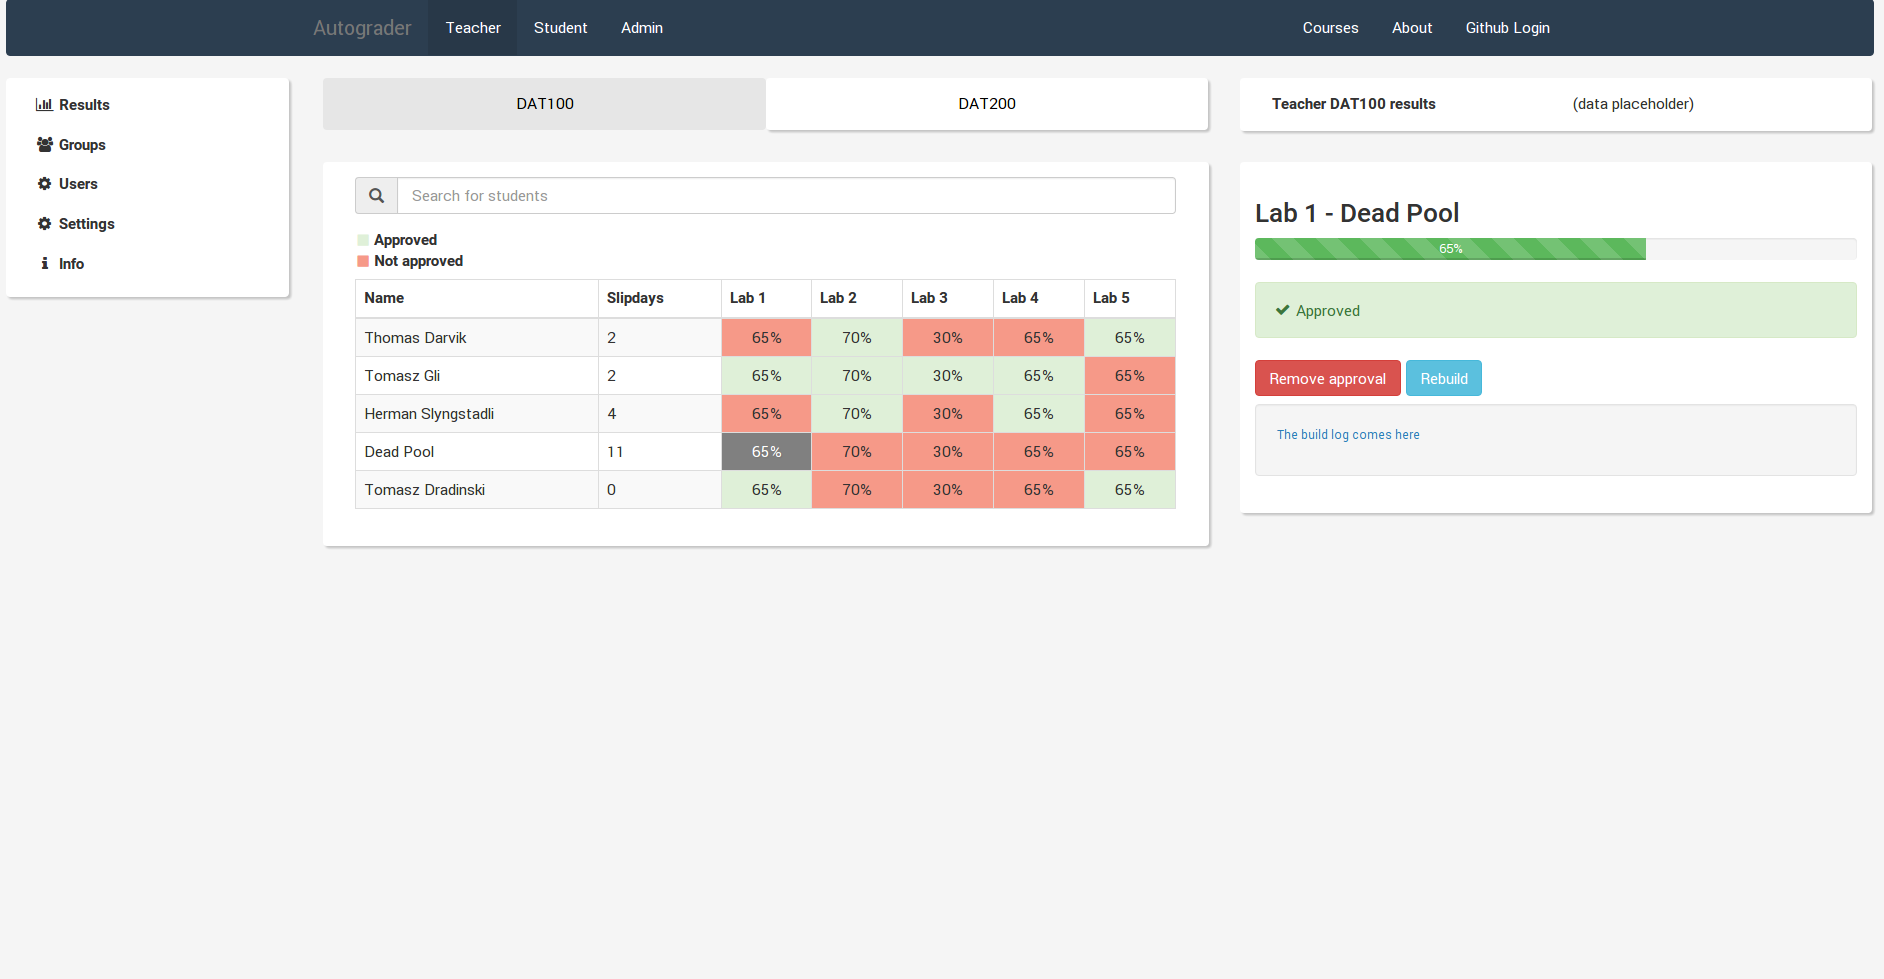
\includegraphics[width=1\linewidth]{./graphs/laboverviewteacher}}
  \caption{The view that teacher sees when looking at all the labs in a given course}
  \label{fig:laboverviewteacher}
\end{figure}
The center section is a table of all the lab results for every student, to the right there is a expanded view of a selected lab (marked with gray).
Simple flowchart represented with MVC style design:
\begin{figure}[h]
\centering
\scalebox{0.9}{% Graphic for TeX using PGF
% Title: /home/tomgli/workspace/github.com/bachopp/thesis/files/chapters/design/graphs/modelmvc.dia
% Creator: Dia v0.97.3
% CreationDate: Wed Apr 20 16:35:36 2016
% For: tomgli
% \usepackage{tikz}
% The following commands are not supported in PSTricks at present
% We define them conditionally, so when they are implemented,
% this pgf file will use them.
\ifx\du\undefined
  \newlength{\du}
\fi
\setlength{\du}{15\unitlength}
\begin{tikzpicture}
\pgftransformxscale{1.000000}
\pgftransformyscale{-1.000000}
\definecolor{dialinecolor}{rgb}{0.000000, 0.000000, 0.000000}
\pgfsetstrokecolor{dialinecolor}
\definecolor{dialinecolor}{rgb}{1.000000, 1.000000, 1.000000}
\pgfsetfillcolor{dialinecolor}
\definecolor{dialinecolor}{rgb}{1.000000, 1.000000, 1.000000}
\pgfsetfillcolor{dialinecolor}
\fill (29.571900\du,2.356000\du)--(29.571900\du,5.957392\du)--(35.666573\du,5.957392\du)--(35.666573\du,2.356000\du)--cycle;
\pgfsetlinewidth{0.100000\du}
\pgfsetdash{}{0pt}
\pgfsetdash{}{0pt}
\pgfsetmiterjoin
\definecolor{dialinecolor}{rgb}{0.000000, 0.000000, 0.000000}
\pgfsetstrokecolor{dialinecolor}
\draw (29.571900\du,2.356000\du)--(29.571900\du,5.957392\du)--(35.666573\du,5.957392\du)--(35.666573\du,2.356000\du)--cycle;
% setfont left to latex
\definecolor{dialinecolor}{rgb}{0.000000, 0.000000, 0.000000}
\pgfsetstrokecolor{dialinecolor}
\node at (32.619236\du,3.956696\du){View};
% setfont left to latex
\definecolor{dialinecolor}{rgb}{0.000000, 0.000000, 0.000000}
\pgfsetstrokecolor{dialinecolor}
\node at (32.619236\du,4.756696\du){LAB LIST};
\definecolor{dialinecolor}{rgb}{1.000000, 1.000000, 1.000000}
\pgfsetfillcolor{dialinecolor}
\fill (8.724400\du,4.733100\du)--(8.724400\du,8.334492\du)--(14.819073\du,8.334492\du)--(14.819073\du,4.733100\du)--cycle;
\pgfsetlinewidth{0.100000\du}
\pgfsetdash{}{0pt}
\pgfsetdash{}{0pt}
\pgfsetmiterjoin
\definecolor{dialinecolor}{rgb}{0.000000, 0.000000, 0.000000}
\pgfsetstrokecolor{dialinecolor}
\draw (8.724400\du,4.733100\du)--(8.724400\du,8.334492\du)--(14.819073\du,8.334492\du)--(14.819073\du,4.733100\du)--cycle;
% setfont left to latex
\definecolor{dialinecolor}{rgb}{0.000000, 0.000000, 0.000000}
\pgfsetstrokecolor{dialinecolor}
\node at (11.771736\du,6.333796\du){Model};
% setfont left to latex
\definecolor{dialinecolor}{rgb}{0.000000, 0.000000, 0.000000}
\pgfsetstrokecolor{dialinecolor}
\node at (11.771736\du,7.133796\du){LABS};
\definecolor{dialinecolor}{rgb}{1.000000, 1.000000, 1.000000}
\pgfsetfillcolor{dialinecolor}
\fill (17.732600\du,4.733100\du)--(17.732600\du,8.334492\du)--(23.827273\du,8.334492\du)--(23.827273\du,4.733100\du)--cycle;
\pgfsetlinewidth{0.100000\du}
\pgfsetdash{}{0pt}
\pgfsetdash{}{0pt}
\pgfsetmiterjoin
\definecolor{dialinecolor}{rgb}{0.000000, 0.000000, 0.000000}
\pgfsetstrokecolor{dialinecolor}
\draw (17.732600\du,4.733100\du)--(17.732600\du,8.334492\du)--(23.827273\du,8.334492\du)--(23.827273\du,4.733100\du)--cycle;
% setfont left to latex
\definecolor{dialinecolor}{rgb}{0.000000, 0.000000, 0.000000}
\pgfsetstrokecolor{dialinecolor}
\node at (20.779936\du,6.333796\du){Controller};
% setfont left to latex
\definecolor{dialinecolor}{rgb}{0.000000, 0.000000, 0.000000}
\pgfsetstrokecolor{dialinecolor}
\node at (20.779936\du,7.133796\du){LABS};
\definecolor{dialinecolor}{rgb}{1.000000, 1.000000, 1.000000}
\pgfsetfillcolor{dialinecolor}
\fill (29.740800\du,8.083100\du)--(29.740800\du,11.684492\du)--(35.835473\du,11.684492\du)--(35.835473\du,8.083100\du)--cycle;
\pgfsetlinewidth{0.100000\du}
\pgfsetdash{}{0pt}
\pgfsetdash{}{0pt}
\pgfsetmiterjoin
\definecolor{dialinecolor}{rgb}{0.000000, 0.000000, 0.000000}
\pgfsetstrokecolor{dialinecolor}
\draw (29.740800\du,8.083100\du)--(29.740800\du,11.684492\du)--(35.835473\du,11.684492\du)--(35.835473\du,8.083100\du)--cycle;
% setfont left to latex
\definecolor{dialinecolor}{rgb}{0.000000, 0.000000, 0.000000}
\pgfsetstrokecolor{dialinecolor}
\node at (32.788136\du,9.683796\du){View};
% setfont left to latex
\definecolor{dialinecolor}{rgb}{0.000000, 0.000000, 0.000000}
\pgfsetstrokecolor{dialinecolor}
\node at (32.788136\du,10.483796\du){LAB DETAILS};
\pgfsetlinewidth{0.100000\du}
\pgfsetdash{}{0pt}
\pgfsetdash{}{0pt}
\pgfsetbuttcap
{
\definecolor{dialinecolor}{rgb}{0.000000, 0.000000, 0.000000}
\pgfsetfillcolor{dialinecolor}
% was here!!!
\pgfsetarrowsend{latex}
\definecolor{dialinecolor}{rgb}{0.000000, 0.000000, 0.000000}
\pgfsetstrokecolor{dialinecolor}
\draw (14.819073\du,6.533796\du)--(17.732600\du,6.533800\du);
}
\pgfsetlinewidth{0.100000\du}
\pgfsetdash{}{0pt}
\pgfsetdash{}{0pt}
\pgfsetmiterjoin
\pgfsetbuttcap
{
\definecolor{dialinecolor}{rgb}{0.000000, 0.000000, 0.000000}
\pgfsetfillcolor{dialinecolor}
% was here!!!
\pgfsetarrowsend{latex}
{\pgfsetcornersarced{\pgfpoint{0.000000\du}{0.000000\du}}\definecolor{dialinecolor}{rgb}{0.000000, 0.000000, 0.000000}
\pgfsetstrokecolor{dialinecolor}
\draw (23.827273\du,5.633448\du)--(26.699586\du,5.633448\du)--(26.699586\du,4.156696\du)--(29.571900\du,4.156696\du);
}}
\pgfsetlinewidth{0.100000\du}
\pgfsetdash{}{0pt}
\pgfsetdash{}{0pt}
\pgfsetmiterjoin
\pgfsetbuttcap
{
\definecolor{dialinecolor}{rgb}{0.000000, 0.000000, 0.000000}
\pgfsetfillcolor{dialinecolor}
% was here!!!
\pgfsetarrowsend{latex}
{\pgfsetcornersarced{\pgfpoint{0.000000\du}{0.000000\du}}\definecolor{dialinecolor}{rgb}{0.000000, 0.000000, 0.000000}
\pgfsetstrokecolor{dialinecolor}
\draw (23.827273\du,7.434144\du)--(26.784036\du,7.434144\du)--(26.784036\du,8.983448\du)--(29.740800\du,8.983448\du);
}}
\pgfsetlinewidth{0.100000\du}
\pgfsetdash{}{0pt}
\pgfsetdash{}{0pt}
\pgfsetmiterjoin
\pgfsetbuttcap
{
\definecolor{dialinecolor}{rgb}{0.000000, 0.000000, 0.000000}
\pgfsetfillcolor{dialinecolor}
% was here!!!
\pgfsetarrowsend{latex}
{\pgfsetcornersarced{\pgfpoint{0.000000\du}{0.000000\du}}\definecolor{dialinecolor}{rgb}{0.000000, 0.000000, 0.000000}
\pgfsetstrokecolor{dialinecolor}
\draw (32.619236\du,2.356000\du)--(32.619236\du,1.306000\du)--(20.779936\du,1.306000\du)--(20.779936\du,4.733100\du);
}}
\pgfsetlinewidth{0.100000\du}
\pgfsetdash{}{0pt}
\pgfsetdash{}{0pt}
\pgfsetmiterjoin
\pgfsetbuttcap
{
\definecolor{dialinecolor}{rgb}{0.000000, 0.000000, 0.000000}
\pgfsetfillcolor{dialinecolor}
% was here!!!
\pgfsetarrowsend{latex}
{\pgfsetcornersarced{\pgfpoint{0.000000\du}{0.000000\du}}\definecolor{dialinecolor}{rgb}{0.000000, 0.000000, 0.000000}
\pgfsetstrokecolor{dialinecolor}
\draw (20.779936\du,8.384944\du)--(20.779936\du,9.434944\du)--(13.295405\du,9.434944\du)--(13.295405\du,8.334492\du);
}}
% setfont left to latex
\definecolor{dialinecolor}{rgb}{0.000000, 0.000000, 0.000000}
\pgfsetstrokecolor{dialinecolor}
\node at (25.285537\du,0.860839\du){User action};
% setfont left to latex
\definecolor{dialinecolor}{rgb}{0.000000, 0.000000, 0.000000}
\pgfsetstrokecolor{dialinecolor}
\node at (25.163142\du,5.225726\du){Update};
% setfont left to latex
\definecolor{dialinecolor}{rgb}{0.000000, 0.000000, 0.000000}
\pgfsetstrokecolor{dialinecolor}
\node at (25.263132\du,8.056646\du){Update};
% setfont left to latex
\definecolor{dialinecolor}{rgb}{0.000000, 0.000000, 0.000000}
\pgfsetstrokecolor{dialinecolor}
\node at (16.168522\du,5.834114\du){Notify};
% setfont left to latex
\definecolor{dialinecolor}{rgb}{0.000000, 0.000000, 0.000000}
\pgfsetstrokecolor{dialinecolor}
\node at (16.168522\du,10.141612\du){Update};
\end{tikzpicture}
}
\caption{Example of how the MVC architecture behaves}
\end{figure}
\\In short, the figure represents only one specific case for implementing certain functionality, there is no general pattern in which data flows through the system, in this case: views signal controller, controller updates model, model notifies about its changes to the controller, then the controller updates the views. This is pretty straight forward, but as the application grows and more components and interactive elements are added it quickly becomes difficult to visualize the flow.
\\Flux was design with simplicity in mind, although the pattern may not appear that different from MVC at first, a key difference is that in Flux the data flow is defined, and every action is forced to the beginning of the system:
\begin{figure}[h]
\centering
\scalebox{0.8}{{% Graphic for TeX using PGF
% Title: E:\workspace\go\src\github.com\bachopp\thesis\files\chapters\design\graphs\modelflux.dia
% Creator: Dia v0.97.2
% CreationDate: Sun Apr 24 14:22:10 2016
% For: Tomasz
% \usepackage{tikz}
% The following commands are not supported in PSTricks at present
% We define them conditionally, so when they are implemented,
% this pgf file will use them.
\ifx\du\undefined
  \newlength{\du}
\fi
\setlength{\du}{15\unitlength}
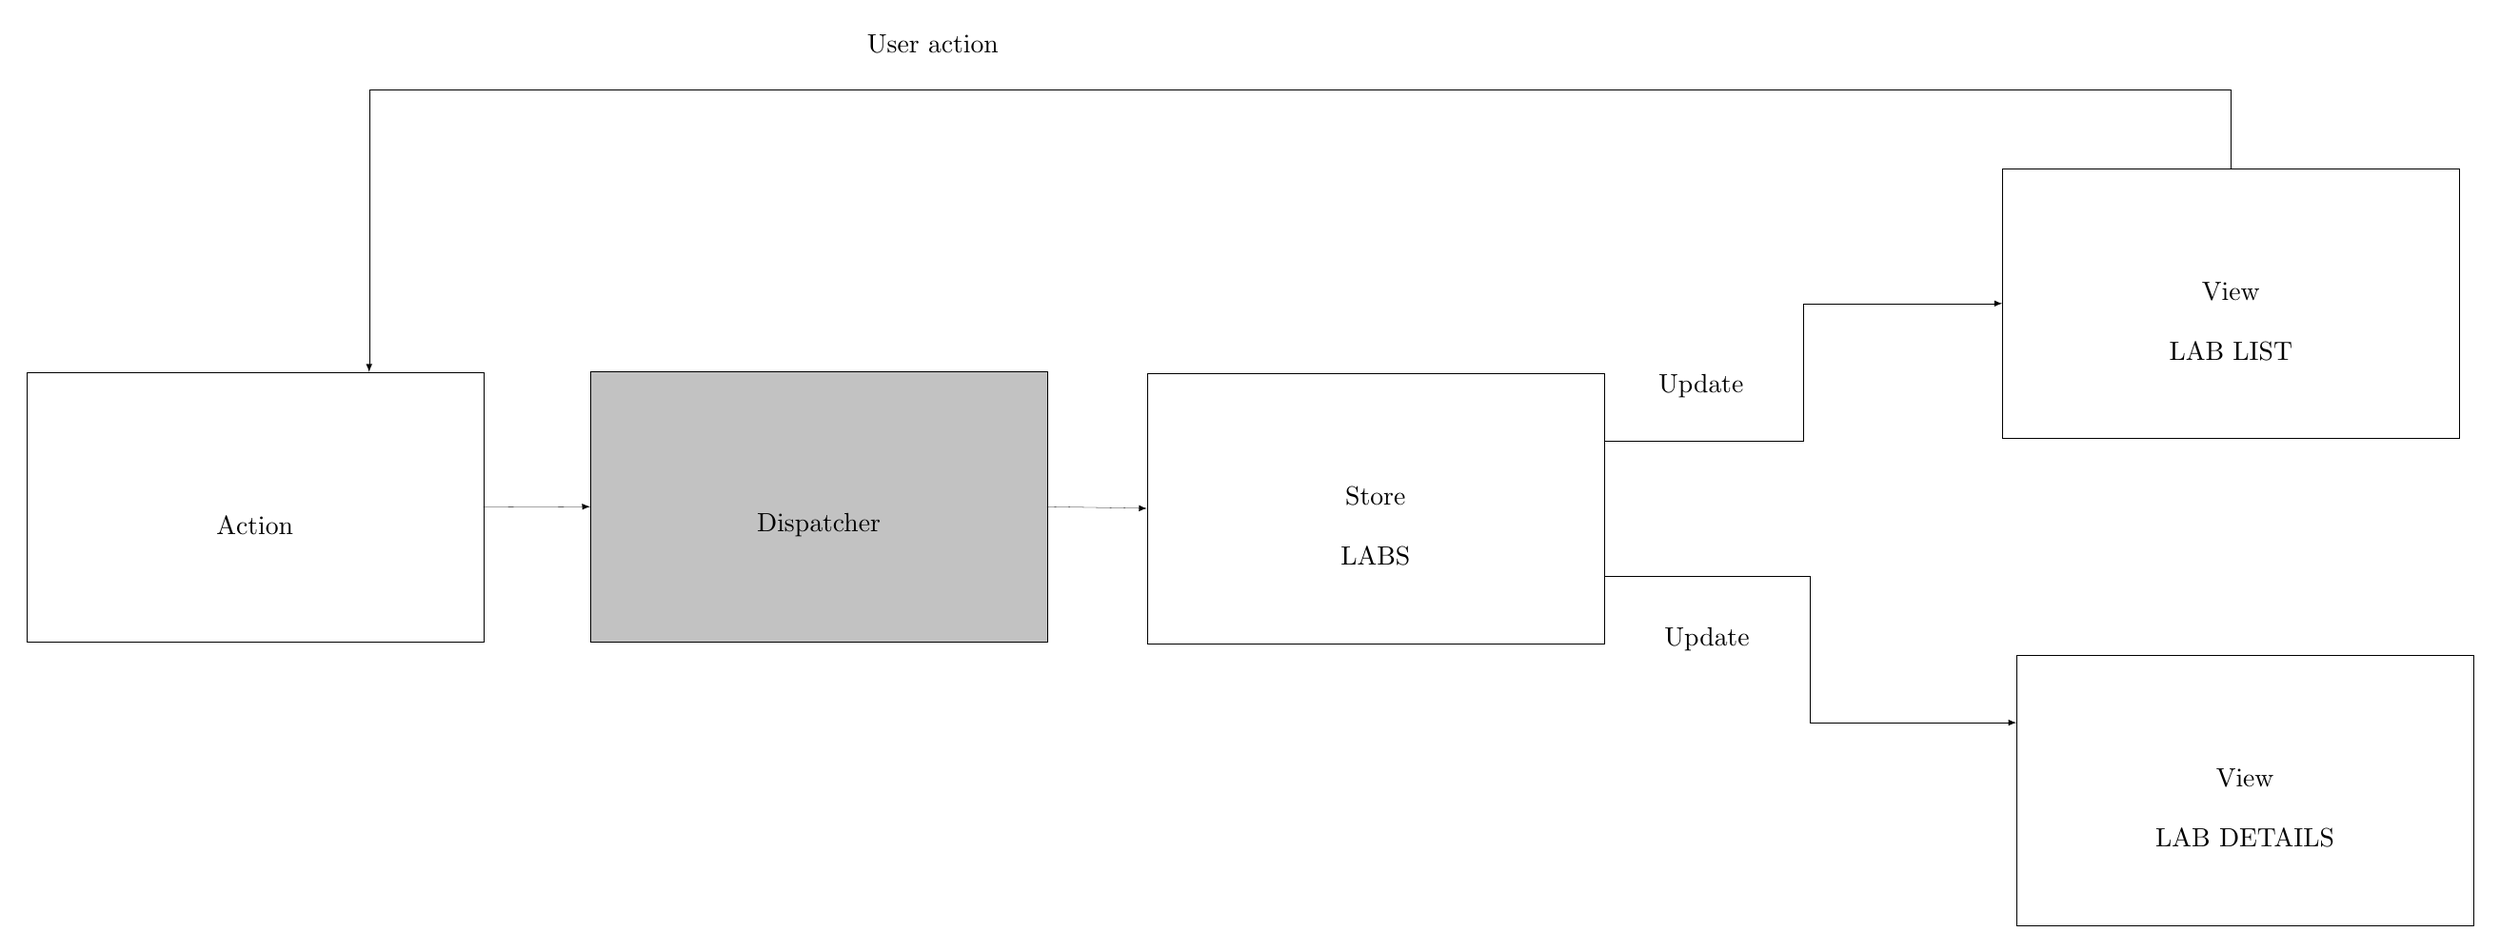
\begin{tikzpicture}
\pgftransformxscale{1.000000}
\pgftransformyscale{-1.000000}
\definecolor{dialinecolor}{rgb}{0.000000, 0.000000, 0.000000}
\pgfsetstrokecolor{dialinecolor}
\definecolor{dialinecolor}{rgb}{1.000000, 1.000000, 1.000000}
\pgfsetfillcolor{dialinecolor}
\definecolor{dialinecolor}{rgb}{1.000000, 1.000000, 1.000000}
\pgfsetfillcolor{dialinecolor}
\fill (30.127000\du,2.450020\du)--(30.127000\du,6.051412\du)--(36.221673\du,6.051412\du)--(36.221673\du,2.450020\du)--cycle;
\pgfsetlinewidth{0.100000\du}
\pgfsetdash{}{0pt}
\pgfsetdash{}{0pt}
\pgfsetmiterjoin
\definecolor{dialinecolor}{rgb}{0.000000, 0.000000, 0.000000}
\pgfsetstrokecolor{dialinecolor}
\draw (30.127000\du,2.450020\du)--(30.127000\du,6.051412\du)--(36.221673\du,6.051412\du)--(36.221673\du,2.450020\du)--cycle;
% setfont left to latex
\definecolor{dialinecolor}{rgb}{0.000000, 0.000000, 0.000000}
\pgfsetstrokecolor{dialinecolor}
\node at (33.174336\du,4.090716\du){View};
% setfont left to latex
\definecolor{dialinecolor}{rgb}{0.000000, 0.000000, 0.000000}
\pgfsetstrokecolor{dialinecolor}
\node at (33.174336\du,4.890716\du){LAB LIST};
\definecolor{dialinecolor}{rgb}{1.000000, 1.000000, 1.000000}
\pgfsetfillcolor{dialinecolor}
\fill (3.767030\du,5.167300\du)--(3.767030\du,8.768692\du)--(9.861703\du,8.768692\du)--(9.861703\du,5.167300\du)--cycle;
\pgfsetlinewidth{0.100000\du}
\pgfsetdash{}{0pt}
\pgfsetdash{}{0pt}
\pgfsetmiterjoin
\definecolor{dialinecolor}{rgb}{0.000000, 0.000000, 0.000000}
\pgfsetstrokecolor{dialinecolor}
\draw (3.767030\du,5.167300\du)--(3.767030\du,8.768692\du)--(9.861703\du,8.768692\du)--(9.861703\du,5.167300\du)--cycle;
% setfont left to latex
\definecolor{dialinecolor}{rgb}{0.000000, 0.000000, 0.000000}
\pgfsetstrokecolor{dialinecolor}
\node at (6.814366\du,7.207996\du){Action};
\definecolor{dialinecolor}{rgb}{0.760784, 0.760784, 0.760784}
\pgfsetfillcolor{dialinecolor}
\fill (11.288700\du,5.160520\du)--(11.288700\du,8.761912\du)--(17.383373\du,8.761912\du)--(17.383373\du,5.160520\du)--cycle;
\pgfsetlinewidth{0.100000\du}
\pgfsetdash{}{0pt}
\pgfsetdash{}{0pt}
\pgfsetmiterjoin
\definecolor{dialinecolor}{rgb}{0.000000, 0.000000, 0.000000}
\pgfsetstrokecolor{dialinecolor}
\draw (11.288700\du,5.160520\du)--(11.288700\du,8.761912\du)--(17.383373\du,8.761912\du)--(17.383373\du,5.160520\du)--cycle;
% setfont left to latex
\definecolor{dialinecolor}{rgb}{0.000000, 0.000000, 0.000000}
\pgfsetstrokecolor{dialinecolor}
\node at (14.336036\du,7.201216\du){Dispatcher};
\definecolor{dialinecolor}{rgb}{1.000000, 1.000000, 1.000000}
\pgfsetfillcolor{dialinecolor}
\fill (18.715500\du,5.183450\du)--(18.715500\du,8.784842\du)--(24.810173\du,8.784842\du)--(24.810173\du,5.183450\du)--cycle;
\pgfsetlinewidth{0.100000\du}
\pgfsetdash{}{0pt}
\pgfsetdash{}{0pt}
\pgfsetmiterjoin
\definecolor{dialinecolor}{rgb}{0.000000, 0.000000, 0.000000}
\pgfsetstrokecolor{dialinecolor}
\draw (18.715500\du,5.183450\du)--(18.715500\du,8.784842\du)--(24.810173\du,8.784842\du)--(24.810173\du,5.183450\du)--cycle;
% setfont left to latex
\definecolor{dialinecolor}{rgb}{0.000000, 0.000000, 0.000000}
\pgfsetstrokecolor{dialinecolor}
\node at (21.762836\du,6.824146\du){Store};
% setfont left to latex
\definecolor{dialinecolor}{rgb}{0.000000, 0.000000, 0.000000}
\pgfsetstrokecolor{dialinecolor}
\node at (21.762836\du,7.624146\du){LABS};
\definecolor{dialinecolor}{rgb}{1.000000, 1.000000, 1.000000}
\pgfsetfillcolor{dialinecolor}
\fill (30.314600\du,8.941950\du)--(30.314600\du,12.543342\du)--(36.409273\du,12.543342\du)--(36.409273\du,8.941950\du)--cycle;
\pgfsetlinewidth{0.100000\du}
\pgfsetdash{}{0pt}
\pgfsetdash{}{0pt}
\pgfsetmiterjoin
\definecolor{dialinecolor}{rgb}{0.000000, 0.000000, 0.000000}
\pgfsetstrokecolor{dialinecolor}
\draw (30.314600\du,8.941950\du)--(30.314600\du,12.543342\du)--(36.409273\du,12.543342\du)--(36.409273\du,8.941950\du)--cycle;
% setfont left to latex
\definecolor{dialinecolor}{rgb}{0.000000, 0.000000, 0.000000}
\pgfsetstrokecolor{dialinecolor}
\node at (33.361936\du,10.582646\du){View};
% setfont left to latex
\definecolor{dialinecolor}{rgb}{0.000000, 0.000000, 0.000000}
\pgfsetstrokecolor{dialinecolor}
\node at (33.361936\du,11.382646\du){LAB DETAILS};
\pgfsetlinewidth{0.100000\du}
\pgfsetdash{}{0pt}
\pgfsetdash{}{0pt}
\pgfsetbuttcap
{
\definecolor{dialinecolor}{rgb}{0.000000, 0.000000, 0.000000}
\pgfsetfillcolor{dialinecolor}
% was here!!!
\pgfsetarrowsend{latex}
\definecolor{dialinecolor}{rgb}{0.000000, 0.000000, 0.000000}
\pgfsetstrokecolor{dialinecolor}
\draw (9.861700\du,6.968000\du)--(11.288700\du,6.961216\du);
}
\pgfsetlinewidth{0.100000\du}
\pgfsetdash{}{0pt}
\pgfsetdash{}{0pt}
\pgfsetbuttcap
{
\definecolor{dialinecolor}{rgb}{0.000000, 0.000000, 0.000000}
\pgfsetfillcolor{dialinecolor}
% was here!!!
\pgfsetarrowsend{latex}
\definecolor{dialinecolor}{rgb}{0.000000, 0.000000, 0.000000}
\pgfsetstrokecolor{dialinecolor}
\draw (17.383373\du,6.961216\du)--(18.715500\du,6.984150\du);
}
\pgfsetlinewidth{0.100000\du}
\pgfsetdash{}{0pt}
\pgfsetdash{}{0pt}
\pgfsetmiterjoin
\pgfsetbuttcap
{
\definecolor{dialinecolor}{rgb}{0.000000, 0.000000, 0.000000}
\pgfsetfillcolor{dialinecolor}
% was here!!!
\pgfsetarrowsend{latex}
{\pgfsetcornersarced{\pgfpoint{0.000000\du}{0.000000\du}}\definecolor{dialinecolor}{rgb}{0.000000, 0.000000, 0.000000}
\pgfsetstrokecolor{dialinecolor}
\draw (24.810173\du,6.083798\du)--(27.468586\du,6.083798\du)--(27.468586\du,4.250716\du)--(30.127000\du,4.250716\du);
}}
\pgfsetlinewidth{0.100000\du}
\pgfsetdash{}{0pt}
\pgfsetdash{}{0pt}
\pgfsetmiterjoin
\pgfsetbuttcap
{
\definecolor{dialinecolor}{rgb}{0.000000, 0.000000, 0.000000}
\pgfsetfillcolor{dialinecolor}
% was here!!!
\pgfsetarrowsend{latex}
{\pgfsetcornersarced{\pgfpoint{0.000000\du}{0.000000\du}}\definecolor{dialinecolor}{rgb}{0.000000, 0.000000, 0.000000}
\pgfsetstrokecolor{dialinecolor}
\draw (24.810173\du,7.884494\du)--(27.562386\du,7.884494\du)--(27.562386\du,9.842298\du)--(30.314600\du,9.842298\du);
}}
\pgfsetlinewidth{0.100000\du}
\pgfsetdash{}{0pt}
\pgfsetdash{}{0pt}
\pgfsetmiterjoin
\pgfsetbuttcap
{
\definecolor{dialinecolor}{rgb}{0.000000, 0.000000, 0.000000}
\pgfsetfillcolor{dialinecolor}
% was here!!!
\pgfsetarrowsend{latex}
{\pgfsetcornersarced{\pgfpoint{0.000000\du}{0.000000\du}}\definecolor{dialinecolor}{rgb}{0.000000, 0.000000, 0.000000}
\pgfsetstrokecolor{dialinecolor}
\draw (33.174336\du,2.450020\du)--(33.174336\du,1.400020\du)--(8.338035\du,1.400020\du)--(8.338035\du,5.167300\du);
}}
% setfont left to latex
\definecolor{dialinecolor}{rgb}{0.000000, 0.000000, 0.000000}
\pgfsetstrokecolor{dialinecolor}
\node at (15.858400\du,0.790717\du){User action};
% setfont left to latex
\definecolor{dialinecolor}{rgb}{0.000000, 0.000000, 0.000000}
\pgfsetstrokecolor{dialinecolor}
\node at (26.105100\du,5.356830\du){Update};
% setfont left to latex
\definecolor{dialinecolor}{rgb}{0.000000, 0.000000, 0.000000}
\pgfsetstrokecolor{dialinecolor}
\node at (26.184500\du,8.726810\du){Update};
\end{tikzpicture}
}}
\caption{General data flow in Flux architecture}
\end{figure}
\\Here a user action is triggered, the dispatcher which is a global central hub of the system, reads what \emph{type} of action is being sent, and notifies the stores about it. Each store represents the data for one or more views. When an action is triggered and reaches store, store then updates itself with the \emph{change} that was associated with the action, when it is done, it notifies the views about the change. Views when they get notified, they get the data from the stores by accessing it through public store getter methods.
This pattern is very scalable, if we were to add more components, by looking at the graph we only need another box, that sends a User action that will further down the graph modify new or the same store. It becomes easier to manage different components, because everything will at some point go through that central hub called the Dispatcher, this is the starting point of every new \emph{state} that the component is in. Since every feature follows same pattern, its easy to grasp the general idea of the application by looking at any particular implementation of any feature, and replicate it with ease. The main difference between Flux and MVC is that flux forces unidirectional dataflow, this might seem unnecessary at first, and it is when it comes to small applications, but nevertheless it simplifies the maintenance of the codebase in the long run.

\subsection{Why Flux}
Flux, like MVC, is just a pattern (think blueprint). It shows how the data will flow in the system. The code must still be written from the ground up in most cases. As said, the data flows unidirectionally, which makes handling states very simple. However, Flux in it self is just another design pattern. Combined with React, the strong sides of the pattern shines. React is state-driven, which is perfect for Flux.
\worry{Write more here..}
